\providecommand{\main}{../../../..}
\documentclass[\main/dresen_thesis.tex]{subfiles}

\begin{document}
  \paragraphNewLine{Scanning Electron Microscopy}
    % The spin-coated nanospheres on silicon substrate are qualitatively viewed by SEM micrographs measured with a Neon Zeiss 40 (\refsec{ch:instruments:laboratoryInstruments:sem}).
    % To obtain cross-sectional views, a piece of a sample is cut on two opposing sides with a diamond cutter and then subsequently broken downward to obtain a clean breaking line, from which SEM measurements can be performed.
    % The micrographs are measured at $5 \unit{kV}$ and the images from the backscattering electrons are shown to obtain a strong contrast.

  \paragraphNewLine{Grazing-Incidence Small-Angle X-ray Scattering}
    % All spin-coated samples were measured at the beam line BM26B \refsec{ch:lss:BM26B} in the ESRF at a wavelength of $\lambda \eq 1.03 \unit{\angstrom}$.
    % For each sample a measurement was performed at a large sample-to-detector distance of $6.54 \unit{m}$ and at a shorter sample-to-detector distance of $2.90 \unit{m}$.
    % The collimation slit is set to $0.3 \times 0.5 \unit{mm^2}$ for each measurement, and every sample is evaluated at an incident angle of $0.2 \unit{^\circ}$.

    % For both samples, a strip of $0.02 \nm^{-1}$ width along the Yoneda band is integrated and compared to the form factor obtained by small-angle X-ray scattering.
    % The scattered intensity for the nanostructure along the Yoneda band is calculated as product of a structure factor and the form factor
    % \begin{align}
    %   I(q) \eq I_0 S(q) |P(q)|^2 + I_\mathrm{bg},
    % \end{align}
    % where $I_0$ is a scaling factor and $I_\mathrm{bg}$ is a incoherent noise background that is not directly associated with the scattering from the nanoparticles.
    % The used form factor $|P(q)|^2$ is hereby given by using the best fit of the nanoparticles from SAXS as determined in \refsec{sec:looselyPackedNS:nanoparticle:sas}.
    % As no calibration measurement has been performed at BM26B, the data is given in the arbitrary count units of the detector.
    % The structure factor for hard spheres of radius $R_\mathrm{HS}$ and with a packing fraction $\eta$ can be calculated analytically in the Percus-Yervick approximation \cite{Percus_1958_Analy, Wertheim_1963_Exact, Pedersen_1997_Analy} and is given by
    % \begin{align}
    %   S(q) &\eq \frac{1}{1 + 24 \eta \frac{G(2 q R_\mathrm{HS})}{2 q R_\mathrm{HS}} }
    % \end{align}
    % with
    % \begin{align}
    %   \begin{split}
    %     G(x)   &\eq \frac{(1 + 2\eta )^2}{(1 - \eta )^4} \cdot \frac{ \sin(x) - x \cos(x)}{x^2}\\
    %            & + \frac {-6 \eta (1 + \eta / 2)^2}{(1 - \eta )^4} \cdot \frac{2 x sin(x) + (2 - x^2) \cos(x) - 2}{x^3}\\
    %            & + \frac{\eta (1 + 2\eta )^2}{2(1 - \eta )^4} \cdot \frac{-x^4 \cos(x) + 4 [(3 x^2 - 6) \cos(x) +(x^3 - 6 x) \sin(x) + 6]}{x^5}\\
    %   \end{split}
    % \end{align}

  \paragraphNewLine{X-Ray Reflectometry}
    % XRR was performed on both SC-IOS-11 and SC-IOS-7 using a Bruker D8 Advanced at the \textsc{Forschungszentrum J\"ulich} \refsec{ch:instruments:laboratoryInstruments:xrr}.
    % The X-ray reflectometer was equipped with a Cu-K$\alpha$ source ($\lambda \eq 1.54 \unit{\angstrom}$) and a $q$-range of $0 \ldots 0.15 \unit{\angstrom^{-1}}$ is evaluated by measuring $2 \theta \eq 0 \ldots 1 \unit{^\circ}$ in $0.005 \unit{^\circ}$ steps over an integrated time of approximately $1 \unit{h}$.
    % The collimation slit on the instrument is $0.2 \unit{mm}$ and both samples have a width of approximately $20 \unit{mm}$.

    % To evaluate the reflectivity, a footprint correction is performed as described in \refsec{ch:methods:xrr}, assuming a equidistributed beam profile.
    % As substrate, the scattering length density of silicon is fixed to the literature value at the given wavelength ($\rho_\mathrm{Si} \eq 20.062 \cdot \unit{10^{-5} \angstrom^{-2}}$) and a spacer layer is allowed for the case of a thin \ch{SiO2} or any organic residues in between silicon and the nanospheres.

    % \begin{figure}[!htbp]
    %   \centering
    %   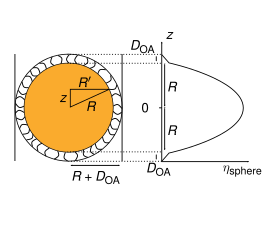
\includegraphics{looselyPackedNP_sphereProfile}
    %   \caption{\label{fig:looselyPackedNP:layerCharacterization:sphereProfile}Evaluation of the cross-section area fraction in comparison to a surrounding cylinder with respect to the height for a sphere with a core radius of $R$ and a oleic acid shell of thickness $D_\mathrm{OA}$.}
    % \end{figure}
    % To model a nanosphere layer, the area fraction of the spheres is needed.
    % The cross-sectional area fraction for a single sphere is given by a parabola, which is trivially derived using the Pythagorean theorem.
    % For a sphere with a surfactant shell, \reffig{fig:looselyPackedNP:layerCharacterization:sphereProfile} can be used to determine the area fraction of the core $\eta_\mathrm{core}$ and the shell $\eta_\mathrm{shell}$, which when evaluated with respect to a surrounding cylinder of radius $R + D_\mathrm{OA}$ are given by
    % \begin{align}
    %   \eta_\mathrm{core} (z)
    %             &\eq \begin{cases}
    %             \eta \frac{R^{2} - z^2}{(R+D_\mathrm{OA})^2}, &\mathrm{for\,}|z|<R \\
    %             0,                                            &\mathrm{else}
    %             \end{cases}\\
    %   \eta_\mathrm{shell} (z)
    %     &\eq \begin{cases}
    %       \eta \frac{2 R D_\mathrm{OA} + D_\mathrm{OA}^2}{(R+D_\mathrm{OA})^2}, &\mathrm{for\,}|z|<R \\
    %       \eta \frac{(R + D_\mathrm{OA})^2 - z^2}{(R+D_\mathrm{OA})^2}, &\mathrm{for\,}R<|z|<R+D_\mathrm{OA} \\
    %       0,                                            &\mathrm{else}
    %     \end{cases}
    % \end{align}
    % where $\eta$ is then the two-dimensional packing density of the surrounding cylinder in the layer.
    % The scattering length density profile $\rho(z)$ of a layer of nanospheres in a matrix of scattering length density $\rho_\mathrm{matrix}$ is then given by
    % \begin{align}
    %   \label{eq:looselyPackedNP:layerCharacterization:sldFromAreaFraction}
    %   \rho(z) \eq \rho_\mathrm{matrix} + (\rho_\mathrm{core} - \rho_\mathrm{matrix}) \eta_\mathrm{core}(z) + (\rho_\mathrm{shell} - \rho_\mathrm{matrix}) \eta_\mathrm{shell}(z),
    % \end{align}
    % where $\rho_\mathrm{core}$ and $\rho_\mathrm{shell}$ are the respective scattering length densities of the core and the shell.

    % This formulation can easily be extended to overlapping nanosphere layers by calculating the sum of the respective area fractions for each layer before determining the SLD by \refeq{eq:looselyPackedNP:layerCharacterization:sldFromAreaFraction}.
    % This procedure is performed for both SC-IOS-11 and SC-IOS-7, where as initial model a stack of nanospheres is given, where each layer is pitched on the vertical axis by $\sqrt{8/3} (R + D_\mathrm{OA})$, which would be the distance of two sphere centers for an ideal close sphere packing.
    % The model is fitted by varying the layer density $\eta$ and a shift from the ideal pitch $\Delta z$ for each layer respectively.
    % The parameters for the nanosphere size, surfactant thickness and scattering length density are used as obtained from SAS, noting that the SLD are readjusted for the different X-ray wavelength at the reflectometer with respect to the small-angle scattering experiments.
    % As roughness model a linearly increasing roughness $\sigma \eq \sigma_0 + \Delta \sigma z$ is used to describe a possibly increasing roughness with stack height.


  \paragraphNewLine{Polarized Neutron Reflectometry}
    % Polarized neutron reflectometry has been performed on SuperADAM at the ILL for all discussed samples at a temperature of $300 \unit{K}$ and at a low temperature of $30 \unit{K}$.
    % The neutron wavelength was selected to $\lambda \eq 5.14 \unit{\angstrom}$
  
  \paragraphNewLine{Vibrating Sample Magnetometry}
    % Yip

\end{document}